\documentclass[a4paper,12pt]{article}
\setlength\textwidth{7in}
\usepackage{amssymb,amsmath}
\usepackage{verbatim,graphicx}
\usepackage{fullpage}
\begin{document}

\begin{titlepage}
\vspace*{2cm}
	\begin{center}
	\large{\textbf{An Efficient File Hierarchy Attribute-Based Encryption Scheme in Cloud Computing}}
	\end{center}
	\vspace{0.5cm}
	\begin{center}
	\small{\textit{A seminar report submitted} \\ \vspace{0.25cm} \textit{to} \\ \vspace{0.25cm}\textbf{MANIPAL UNIVERSITY} \\}
	\end{center}
	\vspace{0.25cm}
	\begin{center}
	\small{\textit{For Partial Fulfillment of the Requirement for the\\ \vspace{0.25cm}Award of the Degree\\ \vspace{0.25cm}of}} \\ \vspace{0.25cm}
	\textbf{Bachelor of Technology} \\  \vspace{0.25cm} \textit{in} \\ \textbf{Information Technology}
	\end{center}
	
	\begin{center}
	\small{\textit{by}} \\
	\textbf{Manali Goel} \\ \textbf{Reg. No. 130911306} \\
	\end{center}

	\begin{figure}[h]
  \begin{center}
	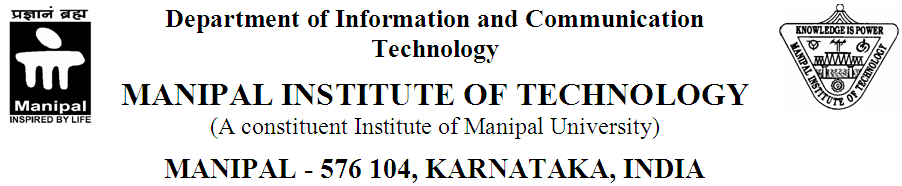
\includegraphics[height=2.8cm]{man}
	\end{center}
	\end{figure}
	\begin{center}
	\textbf{October 2016}
	\end{center}
\end{titlepage}

%\newpage
\begin{abstract}In several distributed systems a user can only access data if user has certain set of credentials or attributes. One method to enforce such policy is to employ a trusted server to store the data and mediate access control. However if server storing the data is compromised then the confidentiality of the data is compromised. Therefore we use Cipher text-Policy Attribute-Based Encryption\cite{1a}. Shared files generally have hierarchical structure which is not explored in Cipher text-Policy Attribute-Based Encryption. 

This article describes an efficient file hierarchy attribute-based encryption scheme  to explore hierarchical structure of shared files in cloud computing.This scheme helps to reduce the computational complexity.  Firstly system definition and basic construction of the file hierarchy attribute-based encryption scheme is proposed that is based on four operations Setup,Key Generation,Encrypt,Decrypt.Then improvement in scheme is proposed and finally using theoretical analysis and experimental simulation the proposed scheme is proved to be highly efficient in terms of encryption and decryption.
\end{abstract}

\newpage
\section{Introduction}Now days people are storing,accessing and sharing their information such as documents, files, data, photos and videos in cloud rather than storing the information locally on a hard disk,removal media,etc. As the technology is expanding the need to protect data from leaking encryption techniques are used. First step to protect data is to ensure authorization. 
Attribute-based encryption scheme ensures authorization. This scheme is public key encryption in which the secret key of a user and cipher text are dependent on the attributes.In such a system, the decryption of a cipher text is possible only if the set of attributes of the user key matches the attributes of the cipher text. \\
There are two types of attribute based encryption scheme : \\ 
1) Key-Policy Attribute-Based Encryption (KP-ABE)\\
2) Cipher text-Policy Attribute-Based Encryption (CP-ABE)

\subsection{Cipher Text-Policy Attribute-Based Encryption Scheme}
In cipher text-policy attribute-based encryption (CP-ABE) a user’s private-key is associated with a set of attributes and a cipher text specifies an access policy over a defined universe of attributes within the system. A user will be ale to decrypt a cipher text, if and only if his attributes satisfy the policy of the respective cipher text.
In CP-ABE scheme each file information is encrypted by different access policies based on the actual need even though files are in same hierarchical structure.

\subsection{File Hierarchy Attribute-Based Encryption Scheme}
Using File Hierarchy Attribute-Based Encryption Scheme(FH-CP-ABE)\cite{2a} we can encrypt multiple hierarchical files with one integrated access structure. Also by this method there is low storage cost and computational complexity in terms of encryption and decryption.

\subsection{Data Sharing In Cloud Computing}
In cloud computing\cite{3a,4a} we have four actors: authority,cloud service provider,data owner and user.\\
1) Authority: It is completely trusted party in Cloud Computing and accepts enrollment from the user.\\
2) Cloud Service Provider: It provide multiple Services to the Client.\\
3) Data Owner: It encrypts the data to be shared/store on cloud and sends the encrypted data to cloud service provider.\\
4) User: Downloads and decrypts the cipher text from cloud service provider.

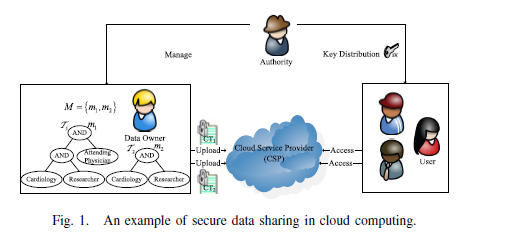
\includegraphics[width=16.5cm,height=14.5cm]{fig1.PNG}
\newpage
\section{Preliminaries}
In this section system definitions and basic constructions is described.
\subsection{Access Structure}
Access Structures are referred as qualified sets.It is used in security where multiple parties work together to obtain a resource.Using access structures people can provide digital signatures. Basically it describes which party should coordinate with whom to get the resources.
\subsection{Bilinear Maps}
 Bilinear map is a function combining elements of two vector spaces to yield an element of a third vector space, and is linear in each of its arguments. Matrix multiplication is an example. In case of encryption Bilinear maps are basically used for pairing based cryptography.
 For this scheme bilinear maps should satisfy three properties like bilinearity, non-degeneracy and compuatability.
\subsection{Hierarchical Access Tree}
In this scheme T is the hierarchical tree that represents and access structure that is divided into different levels(k access levels).\\ \\
Nodes of the tree are represented as ( x, y ) where x denotes the row number and y denotes the column number.\\ \\
This access structure is made by using "OR" and "AND" gates.\\ \\
num\textsubscript{x, y} defines the number of children of node(x, y)\\ \\
k\textsubscript{x,y} denotes the threshold value of node (x, y). If  k\textsubscript{x,y} is 1 then node(x, y) is a non-leaf node and is an "OR" gate but if k\\textsubscript{x,y}=num\textsubscript{x,y} then node (x, y) is a non-leaf node and  "AND" gate.\\ \\
parent\textsubscript{x,y} denotes the parent of the node (x, y).\\
transport nodes are those nodes that contain at least on non-leaf node as their children.\\ \\
index\textsubscript{x,y} returns a unique value associated with the node (x, y).\\ \\
TN-CT(A): It represents number of children of A that are transport nodes.\\ \\
attribute set is the set of leaf nodes.\\
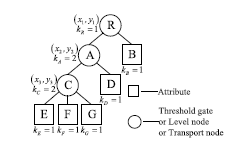
\includegraphics[width=14cm,height=11.5cm]{fig18.PNG}


\subsection{System Definition and Basic Construction}
In this we assume data owner has k files with k access levels and M=\{m\textsubscript{1}, m\textsubscript{2}, ..., m\textsubscript{k}\} are shared in cloud computing.\\ 
\subsubsection{Encryption}
In fig2 a data owner processes the files in the following manner:\\ 
1.)Data owner choose k content keys \{ck\textsubscript{1}, ck\textsubscript{2},.. , ck\textsubscript{k}\} and encrypts files \{m\textsubscript{1}, m\textsubscript{2},..., m\textsubscript{k}\} using symmetric encryption algorithm \{DES,AES \} .\\
2.)Cipher texts are denoted as E\textsubscript{ck}(M)=\{E\textsubscript{ck\textsubscript{1}}(m\textsubscript{1}),...,E\textsubscript{ck\textsubscript{k}}(m\textsubscript{k})\}
3.)Data owner encrypts \{ck\textsubscript{1}, ck\textsubscript{2},.. , ck\textsubscript{k}\} using FH-CP-ABE encryption algorithm and obtains an integrated cipher text of content keys CT.
\subsubsection{Decryption}
1.)User decrypts the cipher text CT and obtain content key by using FH-CP-ABE decryption operation.\\
2.)Then, the user can obtain file by using symmetric decryption algorithm with content key.

\subsubsection{FH-CP-ABE Scheme Operations}
FH-CP-ABE consist of four operations: Setup,Key Generation, Encrypt and Decrypt
\paragraph{Setup}This operation takes a security parameter k as input and outputs public key PK and master secret key MSK.
\paragraph{Key Generation}The operation inputs PK,MSK and a set of attributes S and creates a secret key SK .
\paragraph{Encrypt}The operation inputs PK,\{ck\textsubscript{1}, ck\textsubscript{2},.. , ck\textsubscript{k}\} and a hierarchical access tree A and creates an integrated cipher text of content keys CT.
\paragraph{Decrypt}The algorithm inputs PK, CT which includes an integrated access structure A, SK described by a set of attributes S. If S matches A all content keys can be decrypted. Then corresponding files can be decrypted with content keys by symmetric description algorithm.\\ \\ \\

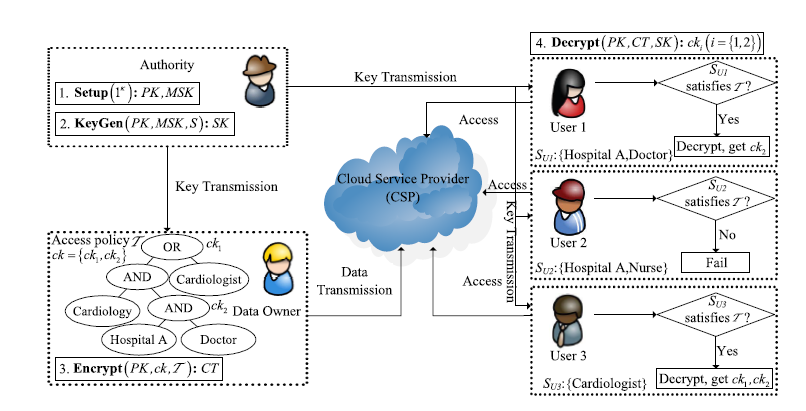
\includegraphics[width=18cm,height=12cm]{fig2.PNG}
Fig 2: An example of FH-CP-ABE scheme in cloud computing
\newpage
\section{The Proposed FH-CP-ABE Scheme}
\subsection{Scheme Construction}
1) Setup : \\
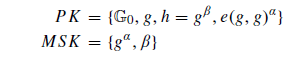
\includegraphics[width=6cm,height=2cm]{fig3.PNG}\\
where PK=Public Key
MSK=Master Secrey Key\\\\
2)Key Generation:\\
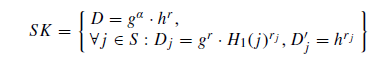
\includegraphics[width=6cm,height=2cm]{fig4.PNG}\\
where SK is Secret Key\\ \\
3)Encrypt Operation:\\ \\
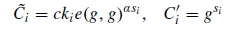
\includegraphics[width=6cm,height=2cm]{fig5.PNG}\\ \\
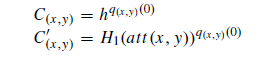
\includegraphics[width=6cm,height=2cm]{fig6.PNG}\\ \\
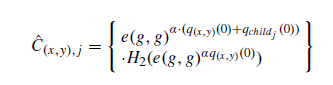
\includegraphics[width=6cm,height=2cm]{fig7.PNG}\\ \\
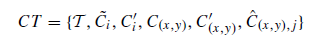
\includegraphics[width=6cm,height=2cm]{fig8.PNG}\\ \\
where CT is integrated cipher text of content keys\\ \\
4)Decrypt Operation:\\ \\
If ( x, y ) is a leaf node decrypt in the following way:\\
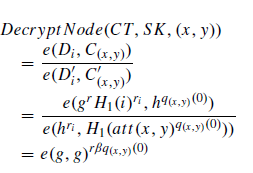
\includegraphics[width=8cm,height=4cm]{fig9.PNG}\\
If ( x, y ) is a non-leaf node decrypt in the following way:\\
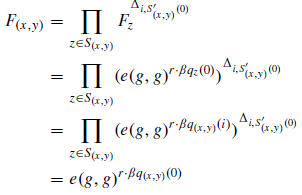
\includegraphics[width=8cm,height=4cm]{fig10.PNG}\\
Procedure to decrypt is :\\
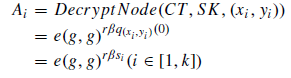
\includegraphics[width=8cm,height=2cm]{fig11.PNG}\\
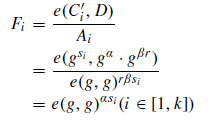
\includegraphics[width=8cm,height=4cm]{fig12.PNG}\\
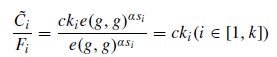
\includegraphics[width=6cm,height=2cm]{fig13.PNG}\\ \\
after this last step is to decrypt the encrypted files using content keys \{ck\textsubscript{1}, ck\textsubscript{2},.. , ck\textsubscript{k}\} using any symmetric decryption algorithm like AES, DES, etc
\subsection{Efficient Scheme of FH-CP-ABE }
In Efficient Scheme of FH-CB-ABE we remove the unwanted transport nodes in order to reduce the computational complexity and storage cost. In the below figure a) part represents the 3 level access structure where we have 9 eligible children threshold gates that are related to transport nodes but using this scheme we reduce these 9 eligible children threshold gates to 3 threshold gates as in b) because nodes B, D, and F do not carry any information regarding the level node.\\
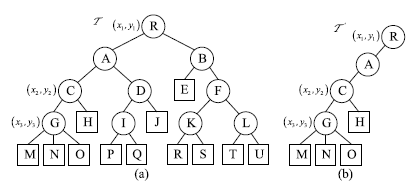
\includegraphics[width=12.5cm,height=12cm]{fig14.PNG}
\subsection{Scheme Features}
1) Computation Cost For Data Owner: \\
As in this scheme we are using a single integrated access structure for the encryption of files therefore here the cost for encryption reduces and hence the efficiency of the data owner is improved.\\
2) Computation Cost For User: Using this scheme the user can decrypt all his authorization files using secret key only once and also the bi linear pairing operation of each common node  is also computed only once. Therefore by using this scheme the decryption cost is also reduced.
\newpage
\section{Security Analysis}
Here two aspects are considered firstly the confidentiality of file cipher text and secondly the confidentiality of content keys that are used for encryption of files.\\ \\
This scheme also proves that no polynomial adversary can selectively break the proposed system.\\ \\
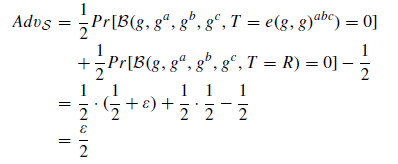
\includegraphics[width=9.5cm,height=5cm]{fig15.PNG}
\newpage
\section{Performance Analysis}
This section describes the efficiency of the proposed scheme by theoretical and practical analysis.\\
\subsection{Theoretical Analysis}
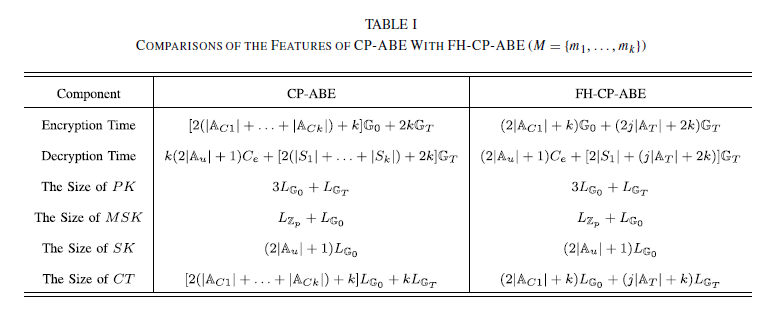
\includegraphics[width=18.5cm,height=11.5cm]{fig16.PNG}
As shown in the above Table1 the length of the Public Key,Master Secret Key and Secret Key is same in both the algorithms but as j is relatively small in FH-CP-ABE Scheme the encryption algorithm is small in FH-CP-ABE Scheme.Hence, theoretically FH-CP-ABE scheme is better than CP-ABE scheme.\\ \\ \\
\subsection{Experimental Results}
The experiments are conducted using Java and all the results are average of more than 10 trials.
Two results were observed firstly the scheme reduces the cost of encryption and decryption and secondly the scheme reduces the storage cost.\\ \\
The experimental results we plotted and graph a) shows the reduction in computational cost of encryption and decryption whereas graph c) shows storage cost of cipher text for various attributes.\\
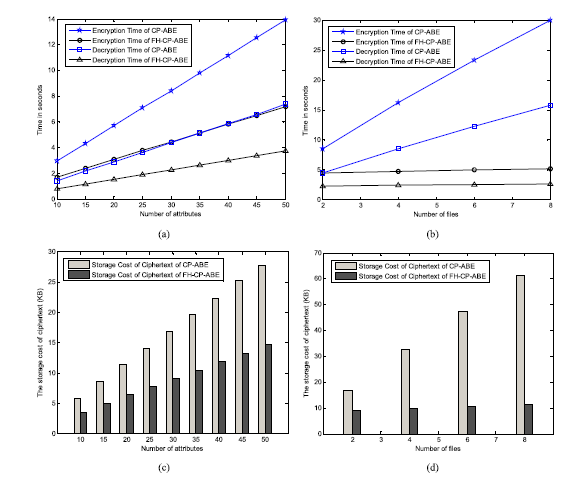
\includegraphics[width=19cm,height=20cm]{fig17.PNG}
\newpage
\section{Conclusion}
In this paper we have extended the CP-ABE scheme and introduced a new scheme FH-CP-ABE which saves the time and computational cost for encryption and decryption also it reduces storage spaces needed for encryption and decryption.This scheme is proved to be secure under DBDH assumptions.Also by using this scheme the user can decrypt all files at once and this scheme provide authorization that is needed for secure transfer of data in cloud computing.\\ \\
In this scheme keys are not user specific they are generated by trusted third party hence any future user can also decrypt the message using the desired attributes and key.As trusted third party is generating the keys authorization is guaranteed here and it becomes difficult for unauthorized users to decrypt the contents of the files.\\ \\
Also this scheme helps in the encryption of hierarchical files with a single integrated structure and the cipher text components related to attributes.Therefore this scheme efficiently share the hierarchical files in cloud computing.










\newpage
\bibliographystyle{IEEEtran}
\bibliography{myref}
	
\end{document}
	 	  